\documentclass[12pt, a4paper]{extarticle}
\usepackage{amsfonts}
\usepackage[T2A]{fontenc}
\usepackage[utf8]{inputenc}
%\usepackage{mathtext}  
\usepackage{amsmath, amsfonts, amssymb}
\usepackage[russian]{babel}
\usepackage[body={17.5cm, 23.5cm},left=3cm, top=2cm, right=2cm]{geometry}
\usepackage{graphicx}
\usepackage{blindtext}
\usepackage{fancyhdr}
\usepackage{graphicx}
\usepackage{ragged2e}
\usepackage{epigraph}
\usepackage{misccorr}  
\usepackage{indentfirst} 
\usepackage{amsmath}
\usepackage{tabularx} 

\usepackage{fancyhdr} 
\usepackage{color}

%\parindent{1.25cm} 
\graphicspath{images/}
\setcounter{tocdepth}{6}
\newcommand{\eps}{\varepsilon}
\newcommand{\re}{\operatorname{Re}}
\newcommand{\im}{\operatorname{Im}}
\DeclareMathOperator{\sgn}{sgn}
\renewcommand{\labelitemi}{$-$}
\renewenvironment{itemize}[1][{---\hfil}]{\begin{list}{#1}{\topsep=0pt\parsep=0pt plus 1pt\itemsep=\parsep\leftmargin=0pt \itemindent=\parindent}\addtolength{\itemindent}{\labelwidth}}{\end{list}}

\numberwithin{equation}{section} 

\newtheorem{attachment}{\hspace{12cm}  Приложение}
\renewcommand{\theattachment}{\Alph{attachment}}
%\renewcommand{\newtheorem}{\Alph{attachment}}
%\newtheorem{Conjecture}{Conjecture}[section]

\usepackage{tocloft}
\renewcommand{\cftsecleader}{\cftdotfill{\cftdotsep}}

\begin{document}
\thispagestyle{empty} 
\medskip 

\begin{center} 
	\textbf{МИНОБРНАУКИ РОССИИ\\ 
		\vspace{0.5cm} 
		Федеральное государственное бюджетное образовательное\\ 
		учреждение высшего образования\\ 
		«Ярославский государственный университет им. П.Г. Демидова»}\\ 
	\vspace{0.5cm} 
	{Кафедра математического моделирования}\\ 
	\vspace{1.5cm} 
	
\end{center}
\begin{flushright} 
	Сдано на кафедру\\
	« 
	\underline{\phantom{aaa}} 
	» 
	\underline{\phantom{aaaaaaaaaaaaa}} 2018 г.\\ 
	Заведующий кафедрой\\
	\underline{\phantom{aaa}д. ф.-м. н., профессор\phantom{aaa}}\\ 
	\vspace{0.1cm} 
	\underline{\phantom{aaaaaaaaaaaaa}} С.А. Кащенко
\end{flushright}
\vspace{3cm} 
\begin{center} 
	Выпускная квалификационная работа\\ 
	\vspace{0.5cm} 
	\textbf{Компьютерное моделирование движения физических объектов}\\ 
	\small{(Направление подготовки бакалавров 01.03.02 Прикладная математика и информатика)}
	\vspace{3cm} 
\end{center} 

\begin{flushright} 
	Научный руководитель\\ 
	\underline{\phantom{aaa}канд. ф-м. н., доцент\phantom{aaa}}\\ 
	\vspace{0.1cm} 
	\underline{\phantom{aaaaaaaaaaaaa}} И.С. Кащенко\\ 
	« 
	\underline{\phantom{aaa}} 
	» 
	\underline{\phantom{aaaaaaaaaaaaa}} 2018 г.\\ 
	\vspace{0.5cm} 
	Студент группы \underline{\phantom{a}ПМИ-42БО\phantom{a}}\\ 
	\vspace{0.1cm} 
	\underline{\phantom{aaaaaaaaaaaaa}} М.А. Погребняк\\ 
	« 
	\underline{\phantom{aaa}} 
	» 
	\underline{\phantom{aaaaaaaaaaaaaa}}2018 г.\\ 
	\vspace{1cm} 
\end{flushright} 
\begin{center} 
	Ярославль 2018 г.
	\vspace{-1cm}  
\end{center} 


\justify 
\setlength{\parindent}{1.25cm} 
\newpage 
\thispagestyle{empty} 
\setcounter{page}{2} 
\section*{Реферат}
\vspace{\baselineskip}	

\newpage

\setcounter{page}{2}

%\thispagestyle{empty} 
\tableofcontents 
\newpage 

\section*{Введение}
\addcontentsline{toc}{section}{Введение}
\epigraph{\textit{Так много в математике физики, как много в физике математики, и я уже перестаю находить разницу между этими науками}}
{-- Альберт Эйнштейн}

\newpage

\section{Постановка задачи} 
  

\newpage
\section{}
Прежде чем составлять, исследовать и математически описывать теорию транспортных потоков, нужно разобраться с самим понятием "транспортный поток". \textbf{Транспортный поток} {\it – это количество единиц транспортных средств одного вида транспорта, проследовавших определённый участок пути в течение установленного промежутка времени} \cite{TrafficFlow}. В качестве транспортного средства рассмотрим автомобиль и будем считать, что все транспортные средства (автомобили) следуют друг за другом. Автомобиль, за которым есть другой автомобиль будем называть \textbf{лидером}, а автомобиль перед которым есть другой автомобиль - \textbf{преследователем}. Причём один и тот же автомобиль может являться одновременно и преследователем для впереди идущего, и лидером для позади идущего рис. \ref{car_following}. 

\begin{figure}[h!]  
	\begin{center}
		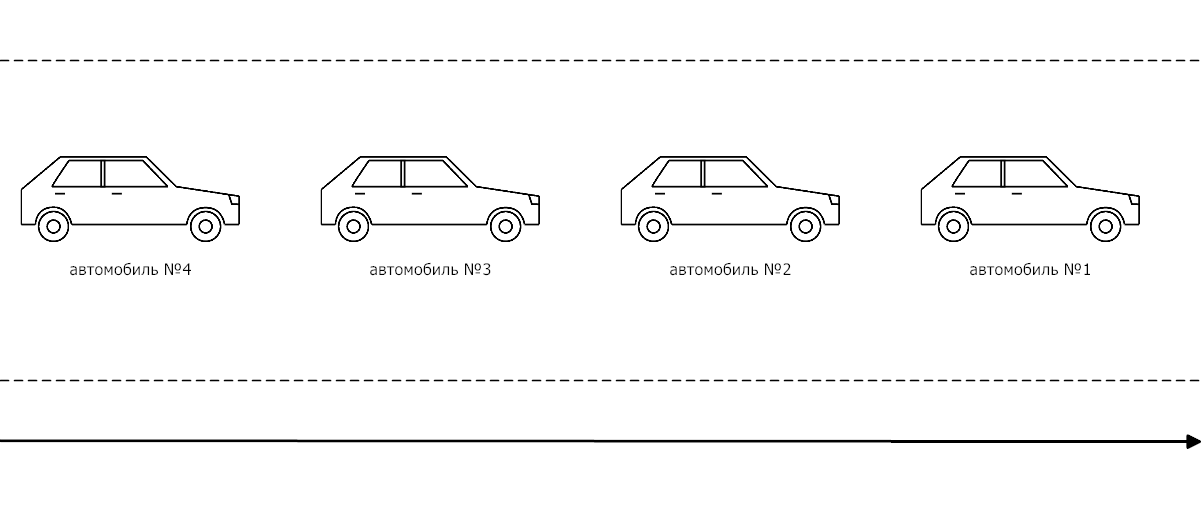
\includegraphics[keepaspectratio,width=160mm,height=70mm]{Images/car_following.png}
	\end{center}
	\caption{Следующие друг за другом автомобили.}
	\label{car_following}
\end{figure}

Теперь рассмотрим парадигму автомобиля, которая основана на очень простом правиле и уже довольно давно известна в литературе, так как автомобили следуют друг за другом, преследователь всегда пытается максимизировать свою скорость с двумя ограничениями: ограничением ускорения и ограничением безопасности. Впервые данная парадигма была высказана ещё в 1975 \cite{GippsModel} и математически выглядит следующим образом:

\begin{equation} \label{following_paradigm}
v_f(t) = \min(v_f^d(t), v_f^s(t))
\end{equation}
где $v_f(t)$ - скорость преследователя в момент времени $t$, $v_f^d(t)$ - максимальная возможная скорость с \textbf{ограничением ускорения} (demand speed), $v_f^s(t)$ - максимальная возможная скорость с \textbf{ограничением безопасности} (supply speed).

Под ограничение ускорения стоит понимать физических ограничения скорости и ускорения транспортного средства, а также комфортные условия для водителя. Оно описывает траекторию транспортного средства, которое свободно разгоняется до максимальной желаемой скорости при отсутствии впереди идущих транспортных средств. Это не всегда постоянное значение: например, оно может зависеть от скорости автомобиля (см. \ref{following_paradigm}). Ограничение безопасности - это то, как траектория транспортного средства зависит от впереди транспортного средства (лидера).

\section{Обобщённая модель следования за лидером}

\begin{equation*}
\ddot{x}(t) = d (\dot{x}(t-\tau)-\dot{x}(t) - \lambda).
\end{equation*}

\begin{equation*}
\begin{cases}
\begin{split}
&\qquad \dot{x}_0 = v_0, \quad x_0(0) = 0, \\
&\ddot{x}_1(t) = d (\dot{x}_0(t-\tau)-\dot{x}_1(t) - \lambda), \\ 
&\qquad \dot{x}_1(0) = 0, \quad x_1(0) = -\lambda, \\
&\ddot{x}_2(t) = d (\dot{x}_1(t-\tau)-\dot{x}_2(t) - \lambda), \\
&\qquad \dot{x}_2(0) = 0, \quad x_2(0) = -2\lambda, \\
&\ldots \\
&\ddot{x}_N(t) = d (\dot{x}_{N-1}(t-\tau)-\dot{x}_N(t) - \lambda), \\
&\qquad \dot{x}_N(0) = 0, \quad x_N(0) = -N\lambda. \\
\end{split}
\end{cases}
\end{equation*}

\begin{equation*}
\begin{cases}
\begin{split}
&\qquad \dot{x}_0 = v_0, \quad x_0(0) = 0, \\
&\ddot{x}_1(t) = d (\dot{x}_0(t-\tau)-\dot{x}_1(t) - \lambda), \\ 
&\qquad \dot{x}_1(0) = 0, \quad x_1(0) = -\lambda, \\
&\ddot{x}_2(t) = d (\dot{x}_1(t-\tau)-\dot{x}_2(t) - \lambda), \\
&\qquad \dot{x}_2(0) = 0, \quad x_2(0) = -2\lambda, \\
&\ddot{x}_3(t) = d (\dot{x}_2(t-\tau)-\dot{x}_3(t) - \lambda), \\
&\qquad \dot{x}_3(0) = 0, \quad x_3(0) = -3\lambda. \\
\end{split}
\end{cases}
\end{equation*}

\begin{table}[h]
	\caption{Физическое значение параметров}
	\label{parameters}
	\begin{center}
		\begin{tabularx}{\textwidth}{p{0.15\linewidth}p{0.85\linewidth}}
			
			\hline
			\rule{0cm}{0,5cm}
			Параметр &  Физическое значение \\ 
			[3pt]\hline
			-- & -- \\
			\hline
		\end{tabularx}
	\end{center}
\end{table}

 
\section{Реализация} 
 

\newpage
\section*{Заключение}
\addcontentsline{toc}{section}{Заключение}

\newpage

\begin{thebibliography}{**}
	\bibitem{TrafficFlow}
	https://spravochnick.ru/logistika/logisticheskie\_potoki/transportnyy\_potok/
	\bibitem{GippsModel}
	Wilson R. E. Gipps’ Model of Highway Traffic. 2002.
	\bibitem{Polygon}
	Выгодский М.Я. Справочник по элементарной математике. 2001.
 	\bibitem{Runge_Kutta}
	 Бахвалов Н.С.  Численные методы. 1975.  
	\bibitem{Refactoring}
	Мартин Ф. Рефакторинг. Улучшение существующего кода. 2008.
\end{thebibliography}

\end{document}